\chapter{Systematic uncertainty calculations}
\epigraph{``I made an error in my computations.''\newline
``Oh? This could be an historic occasion.''}{Mr. Spock and Dr Leonard H. ``Bones'' McCoy, Star Trek: TOS S1E19 Tomorrow Is Yesterday (1967)}
\label{chp:syst}

\section{Introduction}

Determining the systematic uncertainties on the neutron tagging efficiency is important, because even though the value has been validated against Americium-Beryllium calibration data there are still sources of systematic uncertainty that need to be taken into account. Due to the neutron tagging algorithm using the reconstructed neutrino interaction vertex in order to find neutron candidates, it means that there is an association between the neutrino interaction vertex and the neutron capture vertex which is introduced into the neutron tagging efficiency. This is utilised when calculating the systematic uncertainties stemming from secondary interactions (SI), shown later in this Chapter. Therefore uncertainties involving the neutrino interactions, such as neutrino interaction cross section uncertainties and the uncertainty stemming from neutrino flux are calculated. Uncertainties in how particle interactions occur in the simulation are also calculated such as pion final state and secondary interaction uncertainties, nucleon final state interaction and secondary interaction uncertainties and uncertainties on how pions and muons are captured upon $\ch{^{16}O}$. There are also uncertainties stemming from the detector itself which need to be taken into account, such as the uncertainty in PMT gain, detector response from neutrino interaction uncertainties and uncertainties from gamma production from neutron capture detector response. 

\section{Systematic uncertainty calculation methodology}

Systematic uncertainties are calculated in one of two ways: MC re-weighting or MC regeneration. In the MC-reweighting approach, weights are applied to a quantity and the tagging efficiency of the re-weighted MC is extracted. The general methodology is to have the input of a model, defined by a set of parameters, and to vary them one by one and then calculate the reweighted tagging efficiencies. The set of relative discrepancies $\delta_{i}$ are computed from this set of reweighted tagging efficiencies $T_{i}$ and the nominal tagging efficiency $T_{nom}$ using Equation \ref{eq:tageffdiscrep}.
\newline
\begin{equation}
    \delta_{i}=\frac{T_{i}-T_{\text {nom }}}{T_{\text {nom }}} \quad i \in\{\text { parameters }\}
\label{eq:tageffdiscrep}
\end{equation}
\newline

These relative discrepancies $\delta_{i}$ are used to calculate the one individual discrepancy $\delta_{reweighted}$ that would describe the final deviation from the nominal tagging efficiency $T_{nom}$ due to the systematic error. The parameter $\delta_{reweighted}$ describes the model which has been produced through 1$\sigma$ variations of these parameters, therefore the final probability distribution function which describes the deviation from the nominal MC has an assumed Gaussian distribution with the standard deviation being equal to $\delta_{reweighted}$. 
\newline
The other method of estimating a systematic error on the tagging efficiency is Monte Carlo regeneration. This method is used when a single variable is changed, instead of the entire parameter space as with MC re-weighting. Monte Carlo regeneration involves changing a parameter and then re-producing the entire Monte Carlo, and then recalculating the associated tagging efficiency. The deviation of this re-generated Monte Carlo tagging efficiency from the nominal Monte Carlo tagging efficiency is then calculated using Equation \ref{eq:tageffdiscrep}.


The list of systematic errors that affect the tagging efficiency are shown in Table \ref{table:systuncertaintytable}. 

\subsection{Gamma ray detector response}

As mentioned previously, the Americium/Beryllium (Am/Be) source produces a prompt 4.4 MeV gamma ray along with a neutron via Equation \ref{eq:ambe_decay_2}. 

\begin{equation}
    \begin{gathered}
    \alpha{ }^9 \mathrm{Be} \longrightarrow{ }^{12} \mathrm{C}^* \mathrm{n} \\
    { }^{12} \mathrm{C}^* \longrightarrow{ }^{12} \mathrm{C} \gamma(4.4 \mathrm{MeV})
    \end{gathered}
\label{eq:ambe_decay_2}
\end{equation}

In Chapter 6, in order to validate the neutron tagging efficiencies calculated, the tagging efficiency of neutron captures from Am/Be + 8BGO data were also calculated and compared to the Monte Carlo prediction. These efficiencies are shown in Table \ref{table:ambe_tau_chi2} and it is important to understand the errors stemming from the Am/Be + 8BGO neutron capture efficiencies as well. The systematic uncertainties in this Chapter are evaluated by calculating the difference between the nominal tagging efficiency and the tagging efficiency arising from a different process, either a different type of simulation, a different model, or in the case of this uncertainty, a difference in the source of neutrons for neutron capture. Equation \ref{eq:tageffdiscrep} shows how this systematic is quantified; where $\delta_{i}$ is the fractional discrepancy arising from variation in tagging efficiency, $T_{i}$ is the neutron tagging efficiency from the Am/Be + 8BGO data, and $T_{nom}$ is the nominal tagging efficiency of the NCQE MC. 

However, due to Table \ref{table:ambe_tau_chi2} showing three neutron capture efficiencies for the Am/Be data dependent on position, it makes sense to calculate the deviation of each of these from the nominal, using Equation \ref{eq:tageffdiscrep} where $i$ denotes the position of the Am/Be source. Equation \ref{eq:total_ambe_deviation} gives the total deviation of the Am/Be tagging efficiency from the nominal, i.e. the total detector response systematic.

\begin{equation}
    {\delta_{AmBe}}^2= \frac{{\delta_{AmBe}^{Centre}}^2 + {\delta_{AmBe}^{+12z}}^2 + {\delta_{AmBe}^{-12x}}^2}{3} 
\label{eq:total_ambe_deviation}
\end{equation}




\subsection{Neutrino beam flux uncertainty}

The uncertainty on neutrino beam fluxes can be evaluated by looking at the dependence of the tagging efficiency on the flux variations. The beam fluxes for the four flavour modes 
$\left(\nu_{e}, \overline{\nu_{e}}, \nu_{\mu}, \overline{\nu_{\mu}}\right)$ have the fractional uncertainties given for each mode, FHC and RHC. The binned uncertainties are shown in Figure \ref{fig:frac_beam_flux_uncertainty}, and the fractional error on the flux (y-axis) is given by the difference between the replica-target tuned flux and the nominal flux divided by the nominal flux \cite{vladisavljevic_constraining_2018}. The replica tuned flux predictions the uncertainties are derived from were simulated with 1000 JNUBEAM files and the fluxes for Runs 1-9d are combined as shown in Equation \ref{eq:flux_comb}:

\begin{equation}
    \Phi_{\text {combined }}^{\mathrm{SK}}=\frac{1}{\mathrm{~N}_{\text {P.O.T. total }}^{\text {SK }}} \times \sum_{\text {run i }} \mathrm{N}_{\text {P.O.T. run i }}^{\mathrm{SK}} \times \Phi_{\text {run i }}^{\mathrm{SK}}
\label{eq:flux_comb}
\end{equation}

Each individual bin for the flux is increased/decreased by its error, the Monte Carlo re-weighting method is then used to extract the taggging efficiency for each flux bin, and Equation \ref{eq:tageffdiscrep} is used to calculate the fractional uncertainty.



Figure \ref{fig:fluxuncertainty} shows the fractional errors calculated from the reweighted Monte Carlo, with the red bars showing the -1$\sigma$ variation and the blue bars showing the +1$\sigma$ variation. Table \ref{table:systuncertaintytable} contains the value for the total uncertainty resulting from the neutrino beam flux, which was calculated using Equation \ref{eq:summingfluxuncertainty}, where the maximum value between the increased and decreased discrepancy is taken and summed over to produce the final neutrino flux beam uncertainty.
Although there are known correlations between the flux parameters, these are not taken into account, because the impact on the neutron tagging efficiencies is extremely small \cite{akutsu_thesis}.
\newline

\begin{figure}[!htb]
    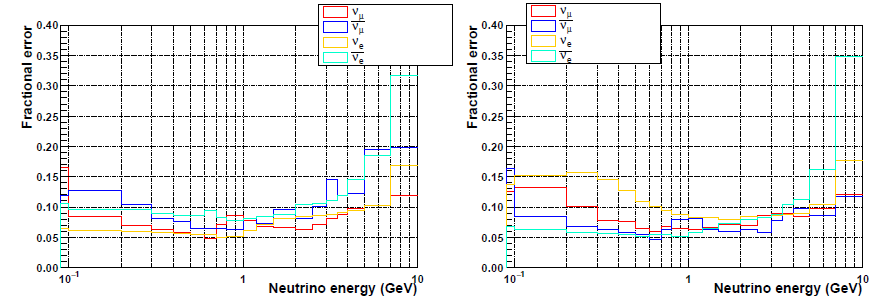
\includegraphics[width=\textwidth]{Figures/frac_beam_flux_uncertainty.png}
    \caption{Fractional uncertainties of beam fluxes, taken from \cite{tn415_fiacob}, for FHC mode. }
    \label{fig:frac_beam_flux_uncertainty}
\end{figure}


\begin{equation}
    \delta_{\nu \text { flux }}=\sum_{i \in\{\text { bins }\}} \max \left[\left|\delta_{i}(+\sigma)\right|,\left|\delta_{i}(-\sigma)\right|\right]
 \label{eq:summingfluxuncertainty}   
\end{equation}

\begin{figure}[!htb]
    \centering
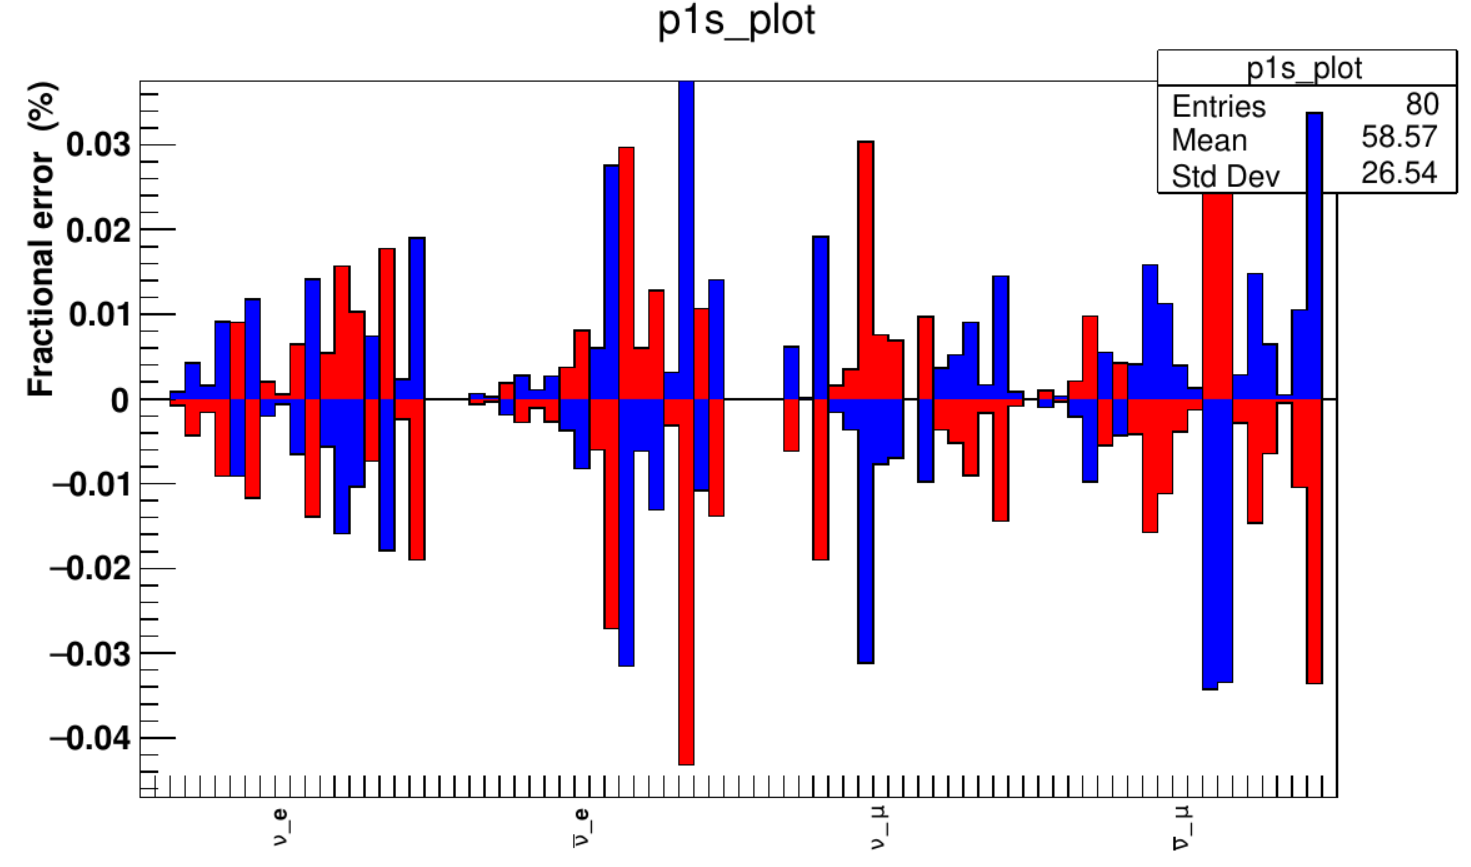
\includegraphics[width=\textwidth]{Figures/flux_uncertainty.png}
\caption{Tagging efficiency fractional uncertainties caused by neutrino beam flux discrepancies associated with neutrino energy in the 0.1 - 10 GeV range. From left to right the sections in this plot are comprised of the beam flux elements of $\left(\nu_{e} \overline{\nu_{e}} \nu_{\mu} \overline{\nu_{\mu}}\right)$ respectively.}
\label{fig:fluxuncertainty}
\end{figure}

\subsection{Neutrino cross section uncertainty}

A group of default neutrino cross section values are used to make up the nominal Monte Carlo from which the tagging efficiency is calculated. The values of the parameters that determine the cross sections are shown in Table \ref{table:xsectable}. Each of the parameter values relate to a specific interaction type and are either a normalisation parameter or a paramater which shows a kinematic dependence. These have been taken from the NIWG model and uncertainties for 2017 oscillation analysis \cite{NIWG_xsec}. \newline

For charged current quasi-elastic interactions, the uncertainty is described by the Fermi momentum of the oxygen nucleus, ($p_{F}^{O}$), the binding energy of the oxygen nucleus, ($E_{B}^{O}$) and the axial mass $M_{A}^{C C Q E}$. The axial mass for CCQE interactions relates to the axial form factor which along with vector form factors is proportional to the cross section of the interactions. For neutrino interactions with correlated nucleons (2p2h), an overall normalisation parameter takes the uncertainty of these interactions into account. For $CC$ and $NC1\pi$ interactions, the uncertainty is described by the isospin background, the axial form factor $C_{A 5}^{R E S}$ which just like for CCQE interactions relates to the axial mass $M_{A}^{R E S}$. For neutral current and charged current interactions (both elastic and inelastic) there are normalisation parameters and energy dependent parameters for the uncertainty to take into account. Finally, for charged current interactions with electron neutrinos, the braking radiation from the lepton in the final state is also considered when calculating the uncertainty and is treated using a normalisation parameter.
\newline

The Monte Carlo re-weighting method is used to reweight the nominal Monte Carlo on an event by event basis with each parameter value being increased and decreased by its uncertainty, where the weights applied are produced by T2KReWeight v1r23, and for each reweighted Monte Carlo the equivalent tagging efficiency value is extracted. Equation \ref{eq:tageffdiscrep} shows how the fractional discrepancies are extracted from the nominal and reweighted tagging efficiency values. Just as with the flux parameters, there are known correlations between the cross-section parameters, but due to the impact on the neutron tagging efficiency being very small these have been ignored. 

Figure \ref{fig:xsecuncertainty} shows the reweighted Monte Carlo fractional uncertainty plotted for the FHC sample. Since this sample contains a lot of NCother interactions, the uncertainty for this interaction type is greater than for the others, however compared to the rest of the systematics in this Chapter, the neutrino cross section uncertainty is very small.

\begin{table}
    \centering
        $\begin{array}{||cccc||}
        \hline & & & \\
        \text { Parameter } & \text { Interaction } & \text { Type } & \text { Value } \\
        \hline
        p_{F}^{O} & \text{CCQE} & { }^{16} \text{O} \text { Fermi momentum } & 225 \pm 31 \text{MeV} / \text{c} \\
        E_{B}^{O} & \text{CCQE} & { }^{16} \text{O} \text { binding energy } & 27 \pm 9 \text{MeV} \\
        M_{A}^{C C Q E} & \text{CCQE} & \text { Axial mass } & 1.2 \pm 0.41 \text{GeV} / \text{c}^{2}\\
        2 p 2 h & 2 \text{p} 2 \text{~h} & \text { Normalization par. } & 1.0 \pm 1.0 \\
        C_{A 5}^{R E S}& \text{CC} \text { and } \text{NC} 1 \pi & \text { Axial form factor } & 1.01 \pm 0.12 \\
        M_{A}^{R E S}  & \text{CC} \text { and NC1 } \pi & \text { Axial mass } & 0.95 \pm 0.15 \text{GeV} / \text{c}^{2} \\
        B G_{A}^{R E S} & \text{CC} \text { and } \text{NC} 1 \pi & \text{I}=1 / 2 \text { continuum background } & 1.3 \pm 0.2 \\
        \text{CC} \text { other } & \text{CC} \text { other } & \text { E-dependent par. } & 0.0 \pm 0.4 \\
        \text{CC} \text { elastic } & \text{CC} \text { elastic } & \text { Normalization par. } & 1.0 \pm 0.3 \\
        \text{NC} \text { other } & \text{NC} \text { other } & \text { E-dependent par. } & 1.0 \pm 0.3 \\
        \text{NC} \text { elastic } & \text{NC} \text {  elastic } & \text { Normalization par. } & 1.0 \pm 0.3 \\
        \text{FS} e^{-} \text {Bremsstrahlung } & \text{CC} \nu_{e} & \text { Normalization par. } & 1.00 \pm 0.03 \\
        \hline
        \end{array}$
        \caption{Neutrino cross section parameters. Taken from \cite{nu_xsec} and \cite{NIWG_xsec}.}
        \label{table:xsectable}
\end{table}


\begin{figure}[!htb]
\centering
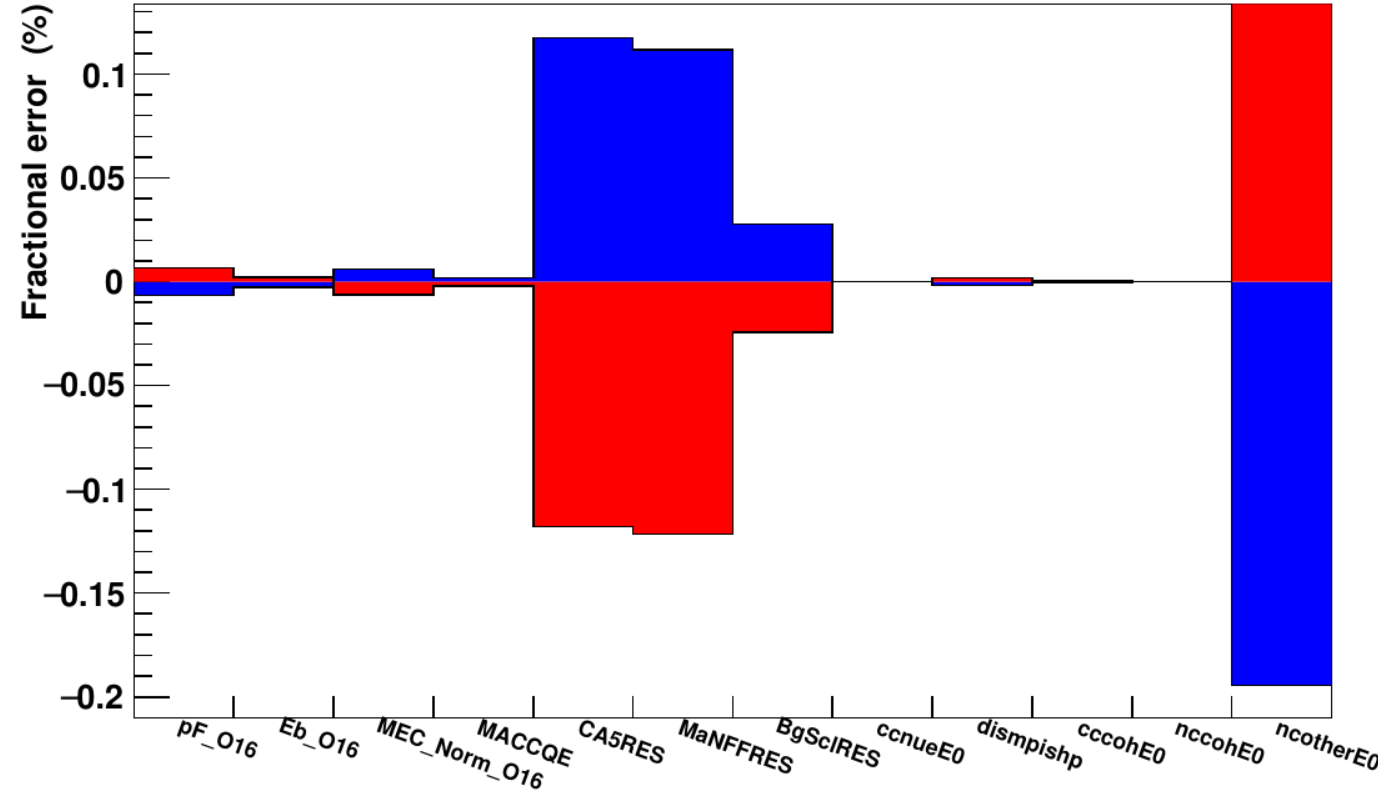
\includegraphics[width=0.8\textwidth]{Figures/xsec_uncertainty.png}
\caption{Tagging efficiency uncertainty caused by the cross-section parameter variations for the FHC mode}
\label{fig:xsecuncertainty}
\end{figure}

\subsection{Pion final state interaction (FSI) and secondary interaction (SI) uncertainties}

Even though this is an analysis concerned with neutral current quasi elastic interactions, pion events are a significant contribution to the background, and as a result it is important to examine the pion interaction uncertainties both for final state interactions and secondary interactions as their trajectories span the detector. 
\newline


The neutrino-nucleus interaction simulator used in this analysis (NEUT) handles pion final state interactions and secondary interactions using a cascade model. This cascade model contains parameters which will have uncertainties on them and these will be tranferred to a possible change in the tagging efficiency.

Depending on the momentum of the pions, different interaction types occur in the model. For pions with a momentum less than 500 MeV, the interactions in place are absorption (ABS), quasi-elastic scattering (QE) and charge exchange (CX).

Absorption occurs when the incident pion is absorbed by the nucleus and no pions remain in the final state. Quasi-elastic (QE) scattering occurs when there is only one pion observed in the final state and it has the same charge as the incident beam. Charge exchange occurs when the charged pion interacts with the nucleus and a single $\pi_{0}$ can be seen in the final state.


For pions with a momentum of greater than 500 MeV, a different set of interactions are used. Inelastic interactions (INEL) can now produce hadrons and replace absorption processes, but quasi-elastic scattering (QEH) and charge exchange (CXH) will still occur. The final state interaction parameters and the pion momentum range they are used in can be seen in Table \ref{table:fsiparameters}. Each parameter scales the relevant very small proabability of the charged pion interaction at every stage of the intra-nuclear cascade, aside from the parameter for charge exchange which scales only the fraction of low momentum QE scattering. 


\begin{table}
\centering
\begin{tabular}{||ccc||}
\hline
$\text { Parameter }$ & $\text { Description }$ & $\text{Momentum Region (MeV/c)}$\\
\hline
$f_{\text{ABS}}$ & $\text{Absorption}$ & $<$ 500 \\
$f_{\text{QE}}$ & $\text { Quasi-elastic scatter }$ & $<$ 500 \\
$f_{\text{CX}}$ & $\text { Single charge exchange }$ & $<$ 500 \\
$f_{\text{QEH}}$ & $\text { Quasi-elastic scatter }$ & $>$ 500 \\
$f_{\text{CXH}}$ & $\text { Single charge exchange }$ & $>$ 500 \\
$f_{\text{INEL}}$ & $\text { Hadron }(\text{N}+\text{n}\pi)$ $\text {production}$ & $>$ 500 \\
\hline
\end{tabular}
\caption{Table showing the pion final state interaction parameters in NEUT and the pion momentum range they are used in, taken from \cite{tn_32}}
\label{table:fsiparameters}
\end{table}



A set of parameter variations which determine a surface in parameter space have been estimated by pion scattering experiments, the values for which are shown in Table \ref{table:fsimodelparameters}. The 1$\sigma$ surface has been explored using the nominal Monte Carlo re-weighting method and the analagous tagging efficiency uncertainty is shown in Equation \ref{eq:tageffdiscrep}, and the uncertainty stemming from the models shown in Table \ref{table:fsimodelparameters} is shown in Figure \ref{fig:fsisiuncertainty}


The pion FSI/SI uncertainty is then calculated using Equation \ref{eq:std_dev_fsisi}, which gives the standard deviation of the fractional uncertainties for each model.

\begin{equation}
\delta_{\pi f s i / s i}=\sqrt{\frac{\sum_i\left(\delta_i-\bar{\delta}\right)^2}{15}} \quad \bar{\delta}=\frac{1}{16} \sum_i \delta_i
\label{eq:std_dev_fsisi}
\end{equation}


\begin{figure}[!htb]
\centering 
    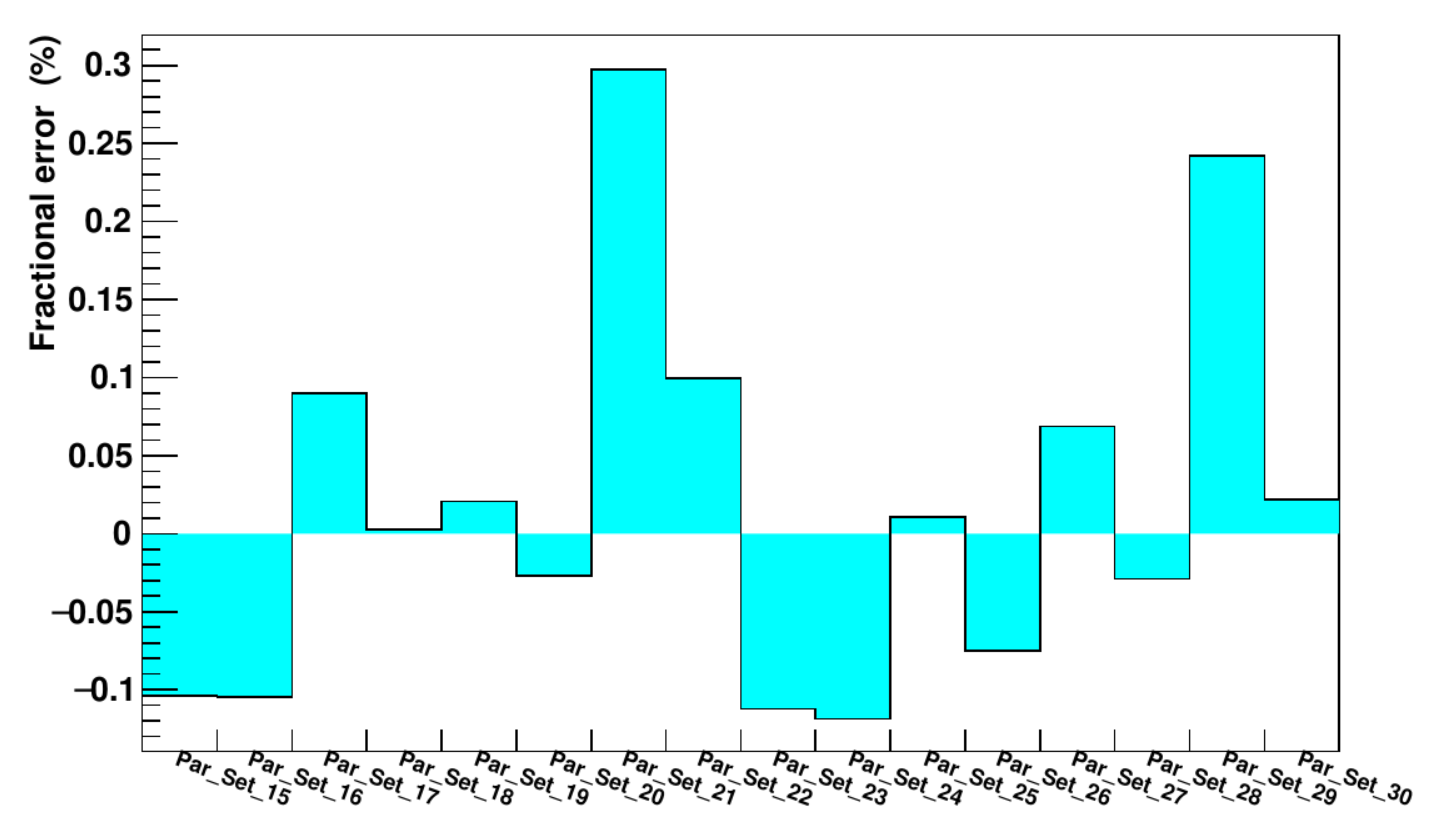
\includegraphics[width=0.8\textwidth]{Figures/fsisi_uncertainty.png}
\caption{Tagging efficiency fractional uncertainty caused by the variation in the FSI/SI model parameters for the FHC mode}
\label{fig:fsisiuncertainty}
\end{figure}

\begin{table}
\centering
\begin{tabular}{||ccccccc||}
\hline
$\text { Set }$ & $\text { ABS }$ & $\text { QE }$ & $\text { CX }$ & $\text { INEL }$ & $\text { QEH }$ & $\text { CXH }$ \\
\hline
    $\text { Nominal }$ & 1.1 & 1.0 & 1.0 & 1.0 & 1.8 & 1.8 \\
    & & & & & & \\
    & 0.7 & 0.6 & 0.5 & 1.5 & 1.1 & 2.3 \\
    & 0.7 & 0.6 & 1.6 & 1.5 & 1.1 & 2.3 \\
    $\text { Hadron production Up }$ & 1.6 & 0.7 & 0.4 & 1.5 & 1.1 & 2.3 \\
    & 1.6 & 0.7 & 1.6 & 1.5 & 1.1 & 2.3 \\
    & 0.6 & 1.4 & 0.6 & 1.5 & 1.1 & 2.3 \\
    & 0.7 & 1.3 & 1.6 & 1.5 & 1.1 & 2.3 \\
    & 1.5 & 1.5 & 0.4 & 1.5 & 1.1 & 2.3 \\
    & 1.6 & 1.6 & 1.6 & 1.5 & 1.1 & 2.3 \\
    & & & & & & \\
    & 0.7 & 0.6 & 0.5 & 0.5 & 2.3 & 1.3 \\
    & 0.7 & 0.6 & 1.6 & 0.5 & 2.3 & 1.3 \\
    & 1.6 & 0.7 & 0.4 & 0.5 & 2.3 & 1.3 \\
    $\text { Hadron production Down }$ & 1.6 & 0.7 & 1.6 & 0.5 & 2.3 & 1.3 \\
    & 0.6 & 1.4 & 0.6 & 0.5 & 2.3 & 1.3 \\
    & 0.7 & 1.3 & 1.6 & 0.5 & 2.3 & 1.3 \\
    & 1.5 & 1.5 & 0.4 & 0.5 & 2.3 & 1.3 \\
    & 1.6 & 1.6 & 1.6 & 0.5 & 2.3 & 1.3\\
\hline
\end{tabular}
\caption{Pion FSI/SI model parameter nominal value and variations grouped according to inelastic hadron production value, taken from \cite{tn_32}.}
\label{table:fsimodelparameters}
\end{table}

\subsection{Nucleon final state interactions}

Uncertainties regarding the nucleon final state interactions can change the number of nucleons knocked out of $\ch{^{16}O}$, therefore how the tagging efficiency is changed due to the variation in nucleon final state interactions needs to be investigated. This uncertainty is extracted using GENIE, a Monte Carlo event generator which contains the INTRANUKE (hA) intranuclear transport model \cite{andreopoulos2010genie}. The uncertainties in the total scattering probability for hadrons inside the target nuclei ($x_{m f p}^{N}$) and the uncertainties in the likelihood of each hadron rescattering method: elastic ($x_{e l}^{N}$), inelastic ($x_{i n e l}^{N}$), charge exchange ($x_{c e x}^{N}$), pion production ($x_{\pi}^{N}$) and absorption ($x_{a b s}^{N}$) are taken into account. The fractional uncertainties for these modes for pions is shown in Table \ref{table:nucleonfsiuncertainties}. 

\begin{table}
\begin{tabular}{||ccc||}
\hline
$\text {Abbreviation}$ & $\text { Description of uncertainty }$  & $\text{Fractional uncertainty}$ \\
\hline
$ x_{m f p}^{N}$ & $\text { Nucleon mean free path (total rescattering probability) }$ & $\pm 20 \%$ \\
$x_{c e x}^{N}$ & $\text { Nucleon charge exchange probability }$ & $\pm 50 \%$ \\
$x_{e l}^{N}$ & $\text { Nucleon elastic reaction probability }$ & $\pm 30 \%$ \\
$x_{i n e l}^{N}$ & $\text { Nucleon inelastic reaction probability }$ & $\pm 40 \%$ \\
$x_{a b s}^{N}$ & $\text { Nucleon absorption probability }$ & $\pm 20 \%$ \\
$x_{\pi}^{N}$ & $\text { Nucleon pion-production probability }$ & $\pm 20 \%$\\
\hline
\end{tabular}
\caption{Nucleon final state interaction parameters of the hA model executed inside GENIE.} 
\label{table:nucleonfsiuncertainties}
\end{table}

A nominal GENIE Monte Carlo sample is generated (different from the previously used NEUT Monte Carlo) and this is shifted using the re-weighting method to a varied GENIE Monte Carlo by individually increasing and decreasing the parameters in Table \ref{table:nucleonfsiuncertainties} by its error. For each shifted Monte Carlo produced, the fractional uncertainty can be written as in Equation \ref{eq:tageffdiscrep}.

The tagging efficiency fractional uncertainties are displayed in Figure \ref{fig:nucleonfsiuncertainty}, showing which parameter from Table \ref{table:nucleonfsiuncertainties} each uncertainty has arisen from.

Because the parameters in Table \ref{table:nucleonfsiuncertainties} are independent, the total uncertainty on the nucleon FSI is calculated by summing the fractional uncertainties on the parameters in quadrature, and then taking the maximum difference between each $\pm \sigma$ pair, as shown in Equation \ref{eq:totalnucleonfsi}.

\begin{equation}
    \delta_{\text{Nucleon FSI}}=\sqrt{\sum_i \max \left[\delta_i^2(+\sigma), \delta_i^2(-\sigma)\right]}
\label{eq:totalnucleonfsi}
\end{equation}

\begin{figure}[!htb]
\centering 
    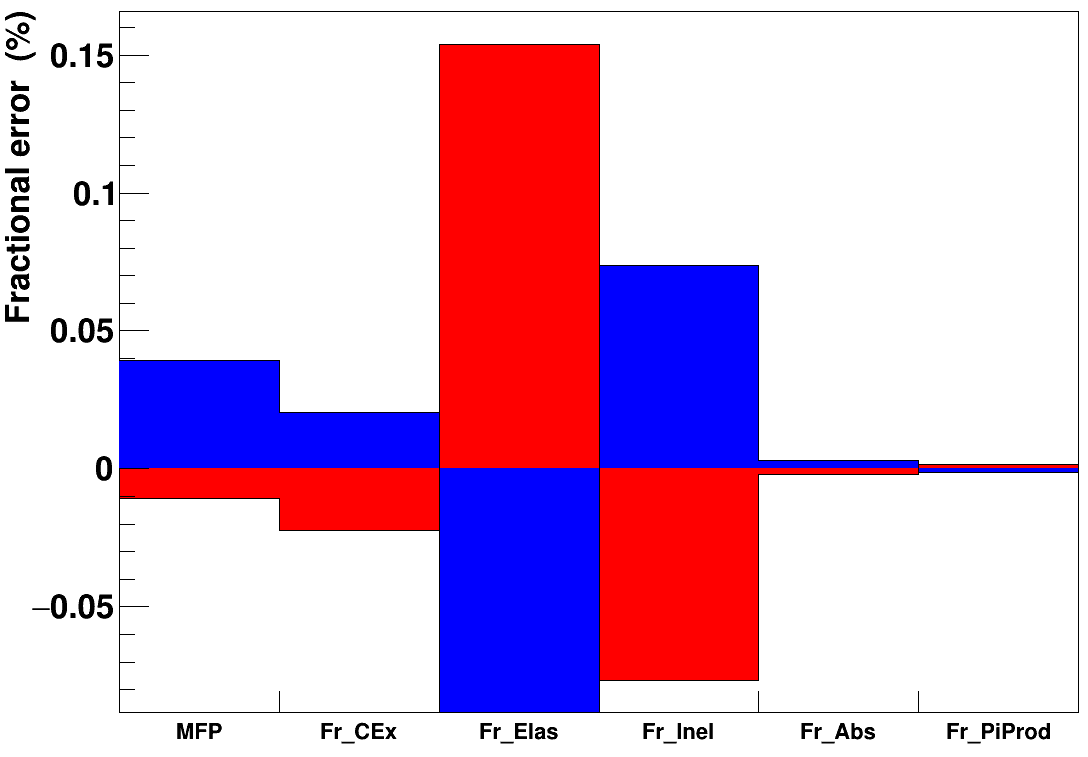
\includegraphics[width=0.7\textwidth]{Figures/nucleonfsi_uncertainty.png}
\caption{Tagging efficiency fractional uncertainties caused by the nucleon final state interaction model parameter variation for the FHC mode}
\label{fig:nucleonfsiuncertainty}
\end{figure}

\subsection{Muon and pion capture on Oxygen-16}

Neutrons are produced from negative muon capture on $\ch{^{16}O}$ as shown in Equation \ref{eq:muoncap}.

\begin{equation}
        \mu^{-}\;\ch{^{16}{O}}\;\longrightarrow\;\nu_{\mu}\;n\;\ch{^{15}{N}}
\label{eq:muoncap}
\end{equation}

Direct neutrons are produced from pion capture on $\ch{^{16}O}$, but also a number of evaporation neutrons that leave the nucleus. For the capture of muons and pions on $\ch{^{16}O}$, the energy spectra of the neutrons produced have been measured: for muons the spectra can range up to 15 MeV, while in the case of pions the spectra can reach up to 100 MeV.


GEANT4 simulates the capture processes for muons and pions, but there are alternate models that can be used: for example, the Chiral Invariant Phase Space (CHIPS) model for muon captures (based on non pertubative QCD) and two different routines for pion capture, one which is based on CHIPS and one based on intra-nuclear cascade.

Because any change in the model can alter the energy spectra of the neutrons, these alternative functions can be used to estimate the fractional uncertainties for the tagging efficiency. This is done by using the MC regeneration method, where the nominal Monte Carlo is regenerated by replacing the default GEANT4 routines with the alternative models. For the alternative muon capture model and the two alternative pion capture models, the fractional discrepancies are shown in Equation \ref{eq:tageffdiscrep}.

Figure \ref{fig:mupicap_uncertainty} shows the fractional uncertainties caused by muon and pion capture on oxygen for each model.

\begin{figure}[!htb]
\centering
    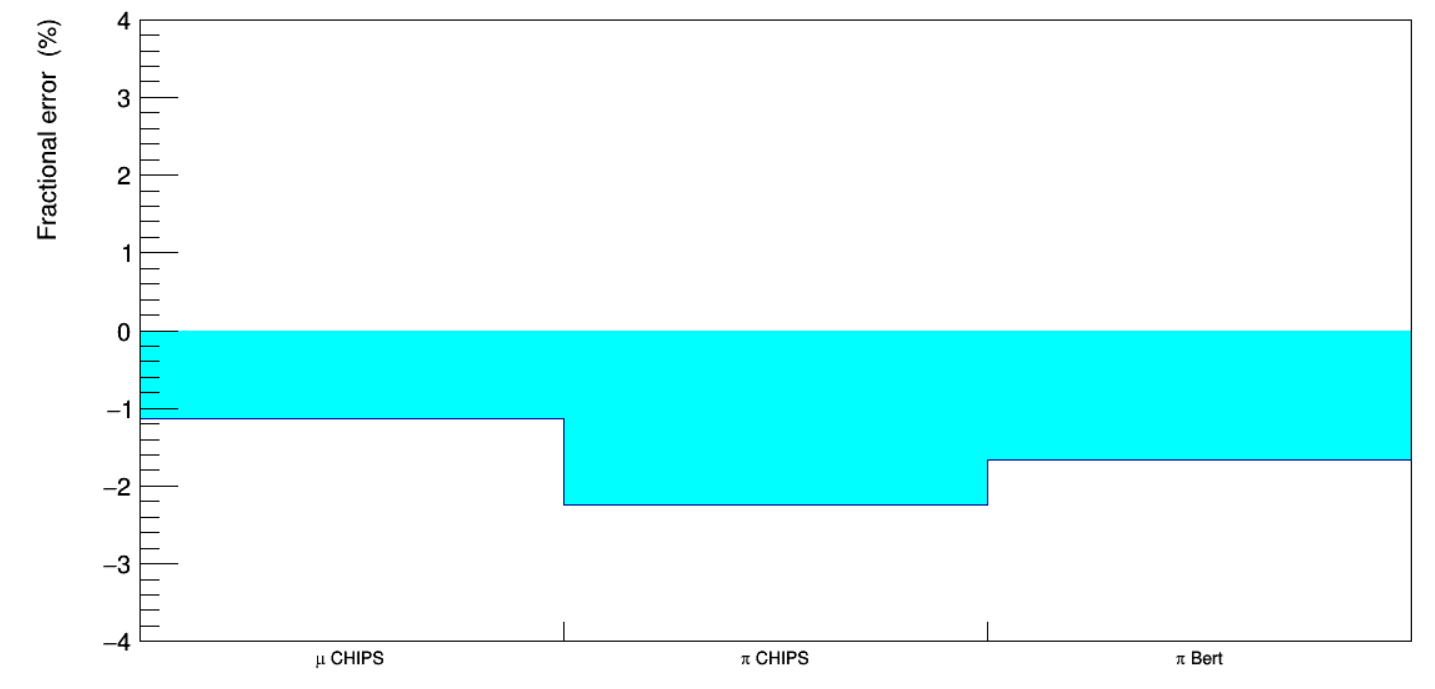
\includegraphics[width=0.7\textwidth]{Figures/mupicap_uncertainty.png}
\caption{Fractional uncertainties in the tagging efficiency caused by muon and pion capture on the muon capture CHIPS model, pion capture CHIPS model and the pion capture Bertini model.}
\label{fig:mupicap_uncertainty}
\end{figure}

The final total muon and pion capture systematic error is summarised in Equation \ref{eq:total_mupicap_error}. Due to the systematic errors $\delta_{muon C H I P S}$, $\delta_{pion C H I P S}$ and $\delta_{pion B e r t}$, (which are the errors due to the muon capture CHIPS model, pion capture CHIPS model and pion capture Bertini model respectively) being independent of one another they can be added in quadrature.

\begin{equation}
    \delta_{\text {muon and pion capture }}=\sqrt{{\delta_{muon C H I P S}}^2 + {\delta_{pion C H I P S}}^2 + {\delta_{pion B e r t}}^2 }
\label{eq:total_mupicap_error}
\end{equation}


\subsection{Nucleon SI}
Uncertainties in how Nucleon SI interactions are modelled can affect the tagging efficiency, due to how these uncertainties can affect the final number of nucleons present in the simulation and how far they travel in the detector medium. There are two Monte Carlo code systems used in order to determine how nucleons travel in the simulation, MICAP and HETC \cite{micap_hetc}. These come as part of GCALOR, used to determine the energy and direction of incident hadrons, leptons and photons \cite{1998gcalor}. MICAP (Monte-Carlo-Ionization-Chamber-Analysis-Program), which simulates interactions based on calculated cross section and angular distributions for secondary particles, and is utilised for neutrons with a kinetic energy below 20 MeV \cite{Zeitnitz:1994bs}. HETC on the other hand, is the High-Energy-Transport-Code, and is responsible for transporting charged hadrons above 20 MeV (up to an energy of 10 GeV) through the detector medium \cite{gabrielhetc}. 

\subsection{MICAP uncertainty calculation}

A library of cross-section data called ENDF \cite{endf} (Evaluated Nuclear Data Files) are used by MICAP to determine what processes the neutrons go through in the detector medium, and their respective cross sections. There are two versions of libraries which are used in evaluating the uncertainty in the tagging efficiency, version B release V (released in 1978) and version B release VIII, released in 2018 \cite{endf8}, \cite{endf82}. There is very little difference between the total neutron on hydrogen cross sections between the two versions of the code, however, in the energy range of 0.1 MeV to 20 MeV, there are differences of up to 40\% in the cross-sections of neutron on oxygen, as shown in Figures \ref{fig:neutron_cross_section_H} and \ref{fig:neutron_cross_section_O}. Both an elastic and inelastic part comprise the total cross-section of a nucleus, and these can affect the way neutrons travel in the simulated detector medium and also the way secondary particles from these interactions are distributed. The way these inelastic processes are simulated depend on the nuclei involved: hydrogen nuclei capture the neutrons in the range ($10^{-11}$, $10^{-7}$) MeV, while neutron captures on oxygen mainly happen on the 4 MeV to 20 MeV energy region. The ENDF/B-VIII library extends the neutron capture energy range for hydrogen to the range ($10^{-11}$, $10^{-4}$) MeV and for captures on oxygen there were differences between ENDF/B-V and ENDF/B-VIII in the 0-10 MeV energy range \cite{akutsu_thesis}.  To calculate the way uncertainties arise from the way MICAP simulates neutron captures, the ENDF-V library is replaced by ENDF-VIII, and the tagging efficiency using this library ($T_{VIII}$) is evaluated from regenerated MC. Equation \ref{eq:MICAP_uncertainty} shows the fractional uncertainty $\delta_{MICAP}$ regarding MICAP.  

\begin{equation}
    \delta_{m c p}=\frac{T_{V I I I}-T_{n o m}}{T_{n o m}}
\label{eq:MICAP_uncertainty}
\end{equation}

\begin{figure}[!htb]
    \centering
    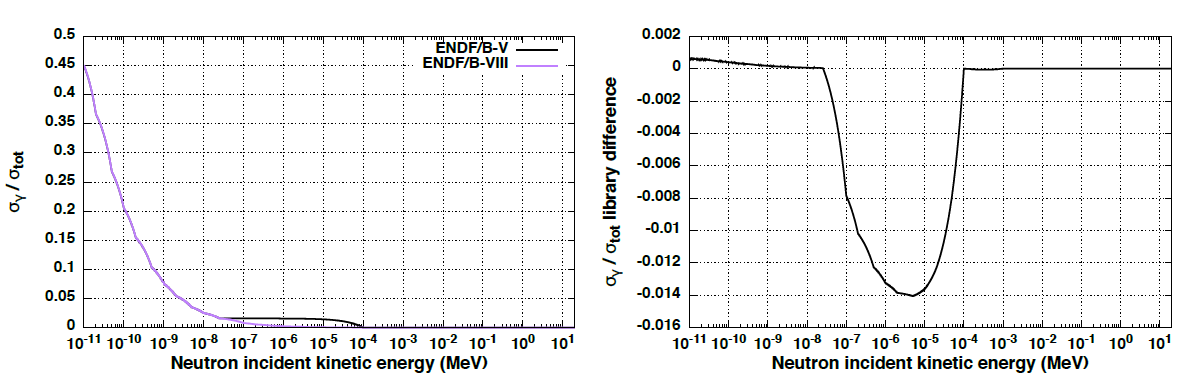
\includegraphics[width=\textwidth]{Figures/neutron_cross_section_endf_H.PNG}
\caption{Left:Fraction of inelastic cross-section for hydrogen for both the ENDF-V and ENDF-VIII libraries. Right: Difference of the fraction of the inelastic cross-section between the two libraries. Taken from \cite{tn415_fiacob}.}
\label{fig:neutron_cross_section_H}
\end{figure}

\begin{figure}[!htb]
    \centering
    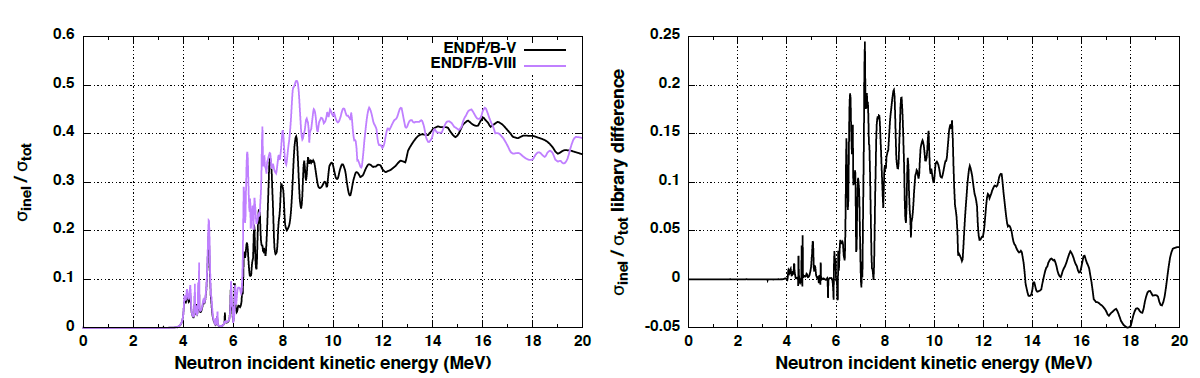
\includegraphics[width=\textwidth]{Figures/neutron_cross_section_endf_O.PNG}
\caption{Left:Fraction of inelastic cross-section for $\ch{^{16}O}$ for both the ENDF-V and ENDF-VIII libraries. Right: Difference of the fraction of the inelastic cross-section between the two libraries. Taken from \cite{tn415_fiacob}.}
\label{fig:neutron_cross_section_O}
\end{figure}

A difference in the inelastic component can change the neutron travel distance, so looking at how changing the Nucleon SI changes the distance between the prompt vertex and the neutron capture vertex is important: this is shown in Figure \ref{fig:ENDF8_syst_error}.

\begin{figure}[!htb]
\centering
    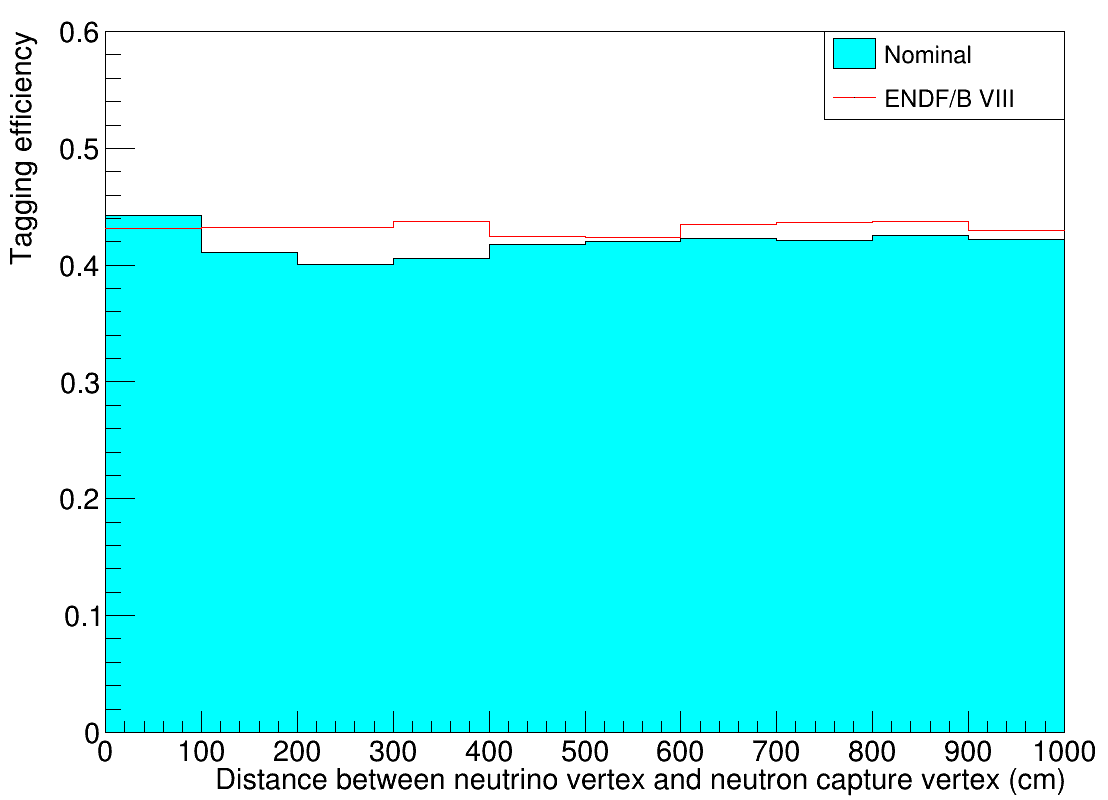
\includegraphics[width=0.7\textwidth]{Figures/endf8_tageff_plot.PNG}
\caption{Tagging efficiency dependence of the true distance between the neutrino and neutron capture vertices between the ENDF V library (used in the nominal MC, shown in cyan) and the ENDF/B VIII library shown in red.}
\label{fig:ENDF8_syst_error}
\end{figure}

\subsection{HETC uncertainty calculation}

Due to there being no experimental data for cross-section calculations on nucleon-oxygen scattering in the energy range at which T2K functions, experimental data of proton-carbon scattering is used to assign error on the cross sections. In the proton-carbon scattering analysis, NEUT was used to evaluate the theoretical cross sections of carbon \cite{hayato_neut}, and this uses cross sections calculated using the Bertini model \cite{bertini_hetc}, which is also used in HETC \cite{hetc_paper}. The comparison of these calculated cross sections to other theoretical calculations as well as to data, showed that the total cross sections calculated by Bertini need to be varied by $\pm$ 30\% in order to be consistent with them. As a result of this, the Monte Carlo is regenerated twice where the free nucleon-nucleon cross sections are scaled by $\pm$ 30\%. Figure \ref{fig:pp_nn_xsec} shows the proton-proton (neutron-neutron) and proton-neutron cross-sections with the shaded area around the line representing the values when the cross sections are scaled by $\pm$ 30\%. Equation \ref{eq:HETC_uncertainty} gives the fractional uncertainty stemming from re-generating the MC with this $\pm$ 30\% scaling, where $\delta_{HETC}(\pm)$ is the error and $T_{HETC}$ is the tagging efficiency of the MC with this scaling.


\begin{figure}[!htb]
\centering
    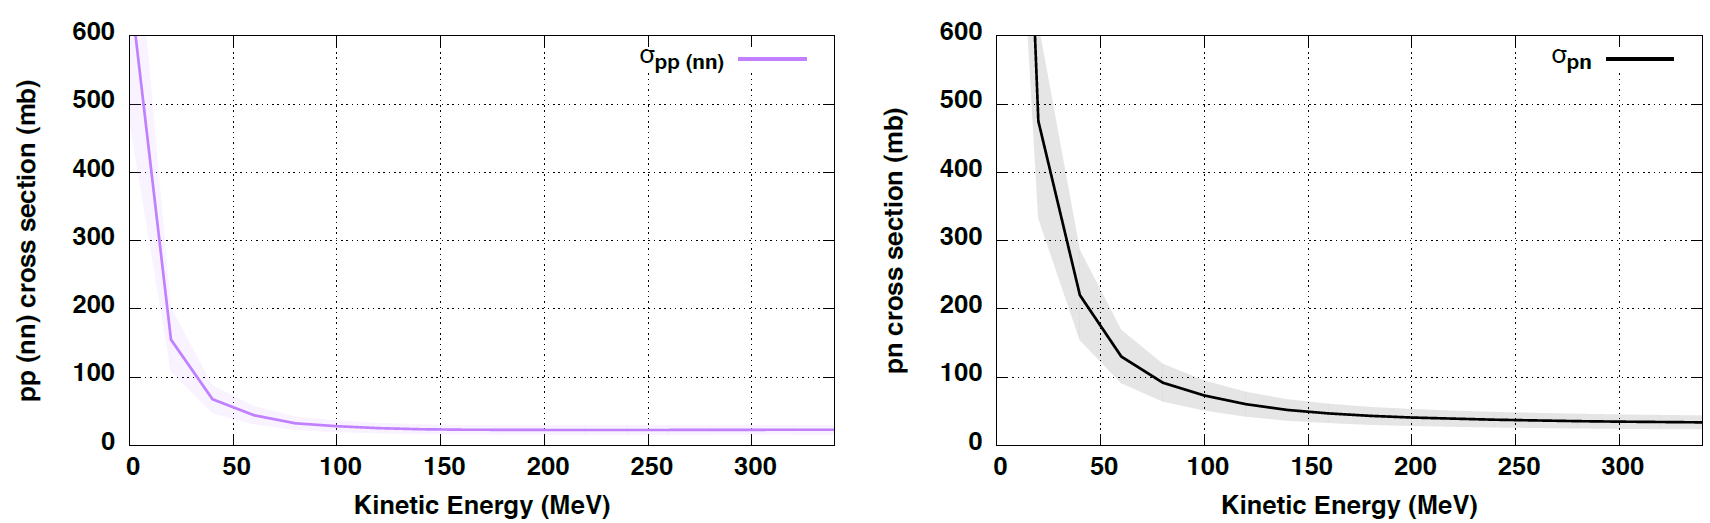
\includegraphics[width=\textwidth]{Figures/pp_nn_xsec.PNG}
\caption{Left: proton-proton (neutron-neutron) cross sections, where the shaded area covers the values which are scaled by $\pm$ 30\%. Right: proton-neutron cross sections, where the shaded area covers the values which are scaled by $\pm$ 30\%. Taken from \cite{tn415_fiacob}.}
\label{fig:pp_nn_xsec}
\end{figure}



\begin{equation}
    \delta_{HETC }(\pm)=\frac{T_{HETC}(\pm)-T_{nom }}{T_{nom }}
\label{eq:HETC_uncertainty}
\end{equation}

Figure \ref{fig:HETC_taggeff_syst} shows the dependence of tagging efficiency on the distance between the prompt vertex and neutron capture vertex for the nominal MC and the scaled cross section by $\pm$ 30\%. 



\begin{figure}[!htb]
\centering
    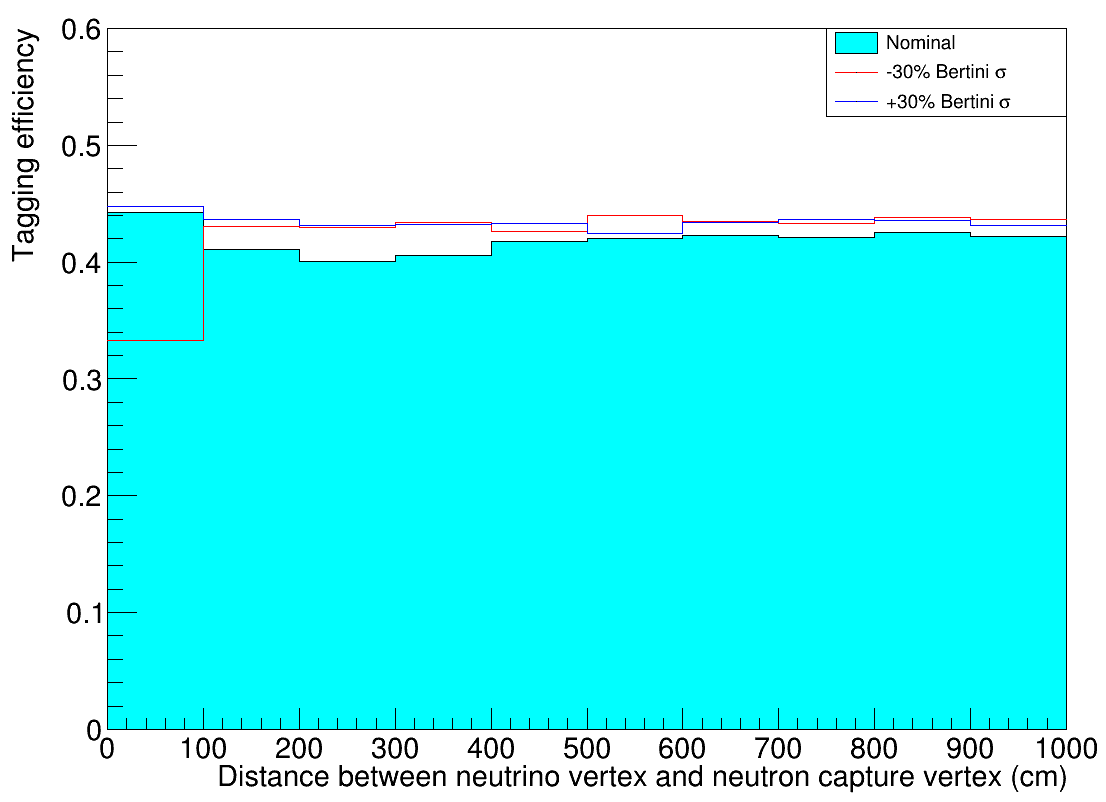
\includegraphics[width=0.7\textwidth]{Figures/hetc_han_syst.PNG}
\caption{Tagging efficiency dependence of the true distance between the prompt vertex and the neutron capture vertex for the nominal MC (cyan) and the $\pm$ 30\% cross section cases.}
\label{fig:HETC_taggeff_syst}
\end{figure}

The fractional discrepancies regarding the HETC codes are not inherently symmetric which is why the positive and negative uncertainties stemming from the Nucleon SI are calculated individually as shown in Equation \ref{eq:nucleon_si_final_error}, and these values are presented in Table \ref{table:systuncertaintytable}.

\begin{equation}
    \begin{aligned}
    & \delta_{\text{Nucleon FSI}}^{+}=\left|\delta_{\text{MICAP}}\right|+\left|\delta_{\text {HETC}}(+\sigma)\right| \\
    & \delta_{\text{Nucleon FSI}}^{-}=\left|\delta_{\text {MICAP}}\right|+\left|\delta_{\text {HETC}}(-\sigma)\right|
    \end{aligned}
    \label{eq:nucleon_si_final_error}
\end{equation}


\subsection{Uncertainty due to PMT gain simulation}

The change in PMT gain over time in the Super-K detector provides a systematic uncertainty for the simulations in this analysis. In SKDETSIM-SKGd the PMT gain drift is modelled by scaling the charge recieved by the PMT according to Equation \ref{eq:PMT_drift_gain}, where $G_{0}$ is the amount of average PMT gain value from June 2017. 

\begin{equation}
    Q \longrightarrow Q \times\left(1+\frac{G(t)-G_0}{G_0}\right)
\label{eq:PMT_drift_gain}
\end{equation}

In addition to the gain changing over time, so does the number of PMT hits due to the gain, and this has to be adjusted by a correction factor of $\alpha$ which has a value of 1.6, shown in Equation \ref{eq:PMT_drift_gain_scaling}. This value is estimated by comparing calibration data and simulations \cite{linyan_thesis}. For $\alpha$ = 1, Equation \ref{eq:PMT_drift_gain_scaling} reduces to Equation \ref{eq:PMT_drift_gain}.


\begin{equation}
    Q \longrightarrow Q \times\left(1+\alpha\frac{G(t)-G_0}{G_0}\right)
\label{eq:PMT_drift_gain_scaling}
\end{equation}

The discrepancies in tagging efficiency for this systematic uncertainty are produced by looking at the fractional uncertainty in tagging efficiencies between $\alpha$ = 1.6 and $\alpha$ = 1, according to Equation \ref{eq:PMT_gain_drift_uncertainty}.

\begin{equation}
    \delta_i=\frac{T_i^{\alpha=1.6}-T_i^{\alpha=1}}{T_i^{\alpha=1}} \quad i \in\{\text { Regeneration points }\}
\label{eq:PMT_gain_drift_uncertainty}
\end{equation}


\subsection{Detector response for neutrino events}
 
The BONSAI fitter output produces parameters that encapsulate the detector repsonse to neutrino events: namely the parameters $E_{rec}$, dwall, effwall, ovaQ, and $\theta_C$. During the selection of NCQE events, cuts are made on these variables in order to give the most plentiful NCQE sample. However, uncertainties on these parameters can modify the amount of NCQE events and affect the position vector of the reconstructed neutrino vertex, and therefore the NTag algorithm, which could have an impact on the tagging efficiency. The errors on these variables are shown in Table \ref{table:det_resp_nu_errors}, and are also provided in TN-374 \cite{tn_374}.

\begin{table}
    \centering
    \begin{tabular}{||cc||}
        \hline Reduction parameter & Uncertainty \\
        \hline$E_{\text {rec }}$ & $\pm 5 \%$ \\
        ovaQ & $\pm 1.5 \%$ \\
        $\theta_C$ & $\pm$ 2 degree \\
        Effwall & $\pm 50 \mathrm{~cm}$ \\
        DWall & $\pm 5 \mathrm{~cm}$ \\
        \hline
        \end{tabular}
\caption{Uncertainties on BONSAI output parameters (taken from \cite{tn_374}).}
\label{table:det_resp_nu_errors}
\end{table}

The nominal Monte Carlo is re-weighted to produce two new Monte Carlo ($\pm$) for each of the BONSAI fitter output parameters, $i$, and the respective tagging efficiencies $T_{i}(\pm\sigma$) are calculated. The fractional uncertainties are given using Equation \ref{eq:tageffdiscrep}, where $i$ represents the Bonai reduction parameter being varied.



Figure \ref{fig:nu_det_syst_error} shows the fractional uncertainties for each parameter. Due to these variables being considered independent of one another, their uncertainties can be summed in quadrature where as usual the maximum is taken between the $\delta(\pm\sigma)$ pairs, shown in Equation \ref{eq:total_nu_det_syst}.

\begin{equation}
    \delta_{\text {$\nu$ response }}=\sqrt{\sum_i \max \left[\delta_i^2(+\sigma), \delta_i^2(-\sigma)\right]}
\label{eq:total_nu_det_syst}
\end{equation}

\begin{figure}[!htb]
    \centering
    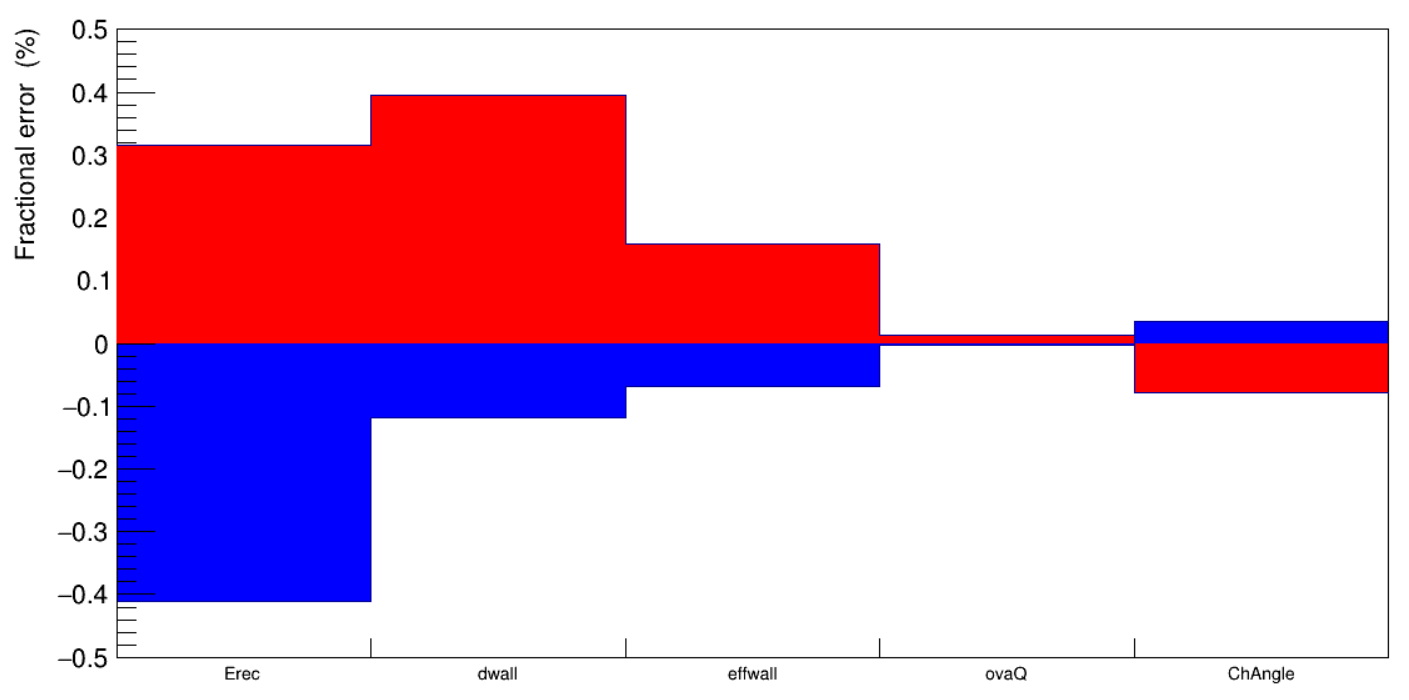
\includegraphics[width=\textwidth]{Figures/nu_det_response.png}
    \caption{Variation in tagging efficiency produced by the error in neutrino detector response parameters (BONSAI output variables). Red: -1$\sigma$ discrepancy. Blue: +1$\sigma$ discrepancy. }
    \label{fig:nu_det_syst_error}
\end{figure}

\newpage


\subsection{Final systematic error}

\begin{table}[htb!]
\centering
\begin{tabular}{||cc||}
    \hline Systematic error & Value $(\%)$ \\
    \hline PMT gain simulation & $\pm$ 3.00 \\
    $\nu$ cross section & $\pm$ 0.30 \\
    $\nu$ beam flux & $\pm$ 0.60 \\
    $\pi$ FSI/SI & $\pm$ 0.10 \\
    Nucleon FSI & $\pm$ 0.20 \\
    Nucleon SI & ${ }_{-5.40}^{+5.40}$ \\
    $\mu$ and $\pi$ capture on ${ }^{16} \mathrm{O}$ & $\pm$ 0.29 \\
    Det. resp. for $\nu$ & $\pm$ 1.36 \\
    Det. resp. for gamma rays & $\pm$ 1.36 \\
    \hline
    \end{tabular}
\caption{Final systematic uncertainties for the tagging efficiency} 
\label{table:systuncertaintytable}
\end{table}


In general the systematic errors associated with the tagging efficiency are as expected: the neutrino cross section and beam flux errors provide only a small contribution to the total systematic error on the tagging efficiency because they have very little impact on the neutron tagging efficiency, and the uncertainty on neutron propagation in Super-Kamiokande. Compared to previous analyses which studied neutron tagging in water at Super-K (\cite{tn415_fiacob}, \cite{akutsu_thesis}), the pion FSI/SI error is small. This could be due to the fact that post the addition of $\mathrm{Gd}_{2}\left(\mathrm{SO}_{4}\right)_{3} \cdot 8 \mathrm{H}_{2} \mathrm{O}$ into the simulation, there are more processes occuring within SKDETSIM due to the additional presence of oxygen, gadolinium and sulphate ions. As a result, the impact that this uncertainty has on the total systematic uncertainty is reduced compared to analyses where these additional nuclei are not present. Similarly, the Nucleon SI uncertainty is also small compared to (\cite{tn415_fiacob}, \cite{akutsu_thesis}), because of the additional interactions occuring on the extra nuclei in the simulation, and therefore the nucleon FSI uncertainty that can alter the number of protons and neutrons knocked out of ${ }^{16} \mathrm{O}$ is lessened. The nucleon SI error is the biggest amongst the uncertainties listed in Table \ref{table:systuncertaintytable}, which is appropriate and in keeping with the results in \cite{tn415_fiacob}, \cite{akutsu_thesis}, as variations in the inelastic cross section for ${ }^{16} \mathrm{O}$ and the uncertainties on the cross sections calculated by the Bertini model which are scaled by $\pm$ 30\% will have a direct impact on the distance between the neutrino interaction vertex and the neutron capture vertex, and therefore a direct impact on the neutron tagging efficiency. The muon and pion capture uncertainties on ${ }^{16} \mathrm{O}$ have smaller values than \cite{akutsu_thesis}, one possible reason for this is the presence of extra gadolinium and sulphate ions in the simulation so that less muons will capture on ${ }^{16} \mathrm{O}$, and as a result the impact on the associated energy spectra of neutrons will be less, so the affect on the neutron tagging efficiency will be less. The neutrino detector response uncertainty is in keeping with the uncertainty evaluated in \cite{tn415_fiacob}, which is understandable as the same errors on the NCQE reduction parameters are used. The detector response from gamma ray uncertainty evaluated by comparisons with Am/Be + 8 BGO data is smaller compared to either of the results from \cite{tn415_fiacob} or \cite{akutsu_thesis} - this makes sense due to the greater compatibility of the NCQE MC neutron tagging efficiency value with the value obtained by comparisons to the Am/Be + BGO data. The uncertainty of the detector response for the neutrinos being the same as the detector response for gamma ray uncertainty is a coincendence ($\pm 1.36$) as these are calculated in two wholly different ways, the former by varying the reduction cut parameters and the latter by comparisons with Am/Be + 8BGO data. The second largest systematic uncertainty in Table \ref{table:systuncertaintytable} comes from the uncertainty in the PMT gain. This value is larger than for \cite{tn415_fiacob} or \cite{akutsu_thesis}, however PMT gain increases over time and as the gain increases so does the neutron tagging efficiency discrepancy due to PMT gain.